
\documentclass[hyperref={pdfpagelabels=false},ngerman]{beamer}

% stop font warning
\let\Tiny=\tiny
\providecommand\thispdfpagelabel[1]{}

\usepackage[english]{babel}
\usepackage{lmodern}
\usepackage[T1]{fontenc}
\usepackage[utf8]{inputenc}
\usepackage{graphicx,import}
\usepackage{feynmp}
\DeclareGraphicsRule{*}{mps}{*}{} 
\DeclareGraphicsExtensions{.pdf}
\usepackage{amsmath,amssymb,amstext,amsfonts} % mathrsfs
\usepackage{array,booktabs,tabularx}
\usepackage{tikz,tikz-uml,pgf-pie}
\usetikzlibrary{shapes,calc,arrows,positioning}
\tikzstyle{block} = [rectangle, draw, text width=7em, text centered, minimum height=2em]
\tikzstyle{arrow} = [draw, -latex, thick]
\tikzstyle{arrow2} = [draw, latex-latex, thick]
\tikzstyle{quark}  = [rectangle, draw, fill=yellow, minimum width=2em, text centered, minimum height=2em]
\tikzstyle{lepton} = [rectangle, draw, fill=red!50, minimum width=2em, text centered, minimum height=2em]
\tikzstyle{gauge}  = [circle   , draw, fill=green , minimum size=2em, inner sep=0pt, text centered]
\tikzstyle{scalar} = [diamond  , draw, fill=blue!40, minimum width=2.3em, text centered, minimum height=2.3em, inner sep=0pt]
\tikzstyle{goldstone} = [diamond, draw, dashed, fill=blue!30, minimum width=2.3em, text centered, minimum height=2.3em, inner sep=0pt]
\tikzstyle{squark}   = [diamond, draw, fill=yellow, minimum width=2.3em, text centered, minimum height=2.3em, inner sep=0pt]
\tikzstyle{slepton}  = [diamond, draw, fill=red!50, minimum width=2.3em, text centered, minimum height=2.3em, inner sep=0pt]
\tikzstyle{gaugino}  = [rectangle, draw, fill=green , minimum size=2em, inner sep=0pt, text centered]
\tikzstyle{higgsino} = [rectangle, draw, fill=blue!40  , minimum width=2em, text centered, minimum height=2em]
\tikzstyle{inert}    = [diamond  , draw, fill=teal!80, minimum width=2.3em, text centered, minimum height=2.3em, inner sep=0pt]
\tikzstyle{inertino} = [rectangle, draw, fill=teal!80, minimum width=2em, text centered, minimum height=2em]
\tikzstyle{graviton} = [regular polygon, regular polygon sides=5, draw, fill=orange!80, minimum width=2em, text centered, minimum height=2em]
\tikzstyle{gravitino} = [regular polygon, regular polygon sides=8, draw, fill=orange!80, minimum width=2em, text centered, minimum height=2em]
\tikzstyle{phantom}  = [rectangle, minimum width=2em, text centered, minimum height=2em]
\usepackage{slashed}
\usepackage{fixltx2e} % textsubscript
\usepackage{multirow}
\usepackage{tcolorbox}
\usepackage{pifont}
\usepackage{xspace}
\usepackage{hyperref}
\hypersetup{colorlinks,linkcolor=,urlcolor=blue}
\usepackage{listings}
\lstset{breaklines=true,
  breakatwhitespace=true,
%  numbers=left,
  numberstyle=\tiny,
  stepnumber=1,
  basicstyle=\ttfamily\footnotesize,
  commentstyle=\ttfamily\color{gray},
  postbreak={\mbox{{$\hookrightarrow$}}\space\space},
  breakindent=10pt,
  breakautoindent=false,
  showspaces=false,
  showstringspaces=false,
  frame=single}

\definecolor{darkgreen}{RGB}{0,176,0}

\newcommand{\cmark}{\ding{51}}%
\newcommand{\xmark}{\ding{55}}%
\newcommand{\fmfvcenter}[1]{\;\vcenter{\hbox{\fmfreuse{#1}}}\;}
\newcommand{\eh}[1]{\,\mathsf{#1}}
\newcommand{\ok}{\textcolor{darkgreen}{\cmark}}
\newcommand{\notok}{\textcolor{red}{\xmark}}
\newcommand{\maybe}{\textcolor{gray}{\cmark}}
\newcommand{\meh}{\textcolor{gray}{\textbf{\huge\lower.1em\hbox{-}}}}
\newcommand{\Lagr}{\mathcal{L}}
\newcommand{\MS}{\ensuremath{M_S}}
\newcommand{\mathi}{\mathsf{i}}
\newcommand{\mycite}[1]{\ensuremath{\text{\textcolor{darkgray}{\tiny [#1]}}}}
\newcommand{\bigcite}[1]{\textcolor{darkgray}{[#1]}}
\newcommand{\dimrep}[1]{\mathbf{#1}}
\newcommand{\dimrepadj}[1]{\mathbf{\overline{#1}}}
\newcommand{\ESSM}{E\textsubscript{6}SSM}
\newcommand{\CESSM}{CE\textsubscript{6}SSM}
\DeclareMathOperator{\tildeRe}{\widetilde Re}
\DeclareMathOperator{\sign}{sign}
\DeclareMathOperator{\re}{Re}
\DeclareMathOperator{\im}{Im}
\renewcommand{\emph}[1]{\textbf{\textcolor{darkblue}{#1}}}
\newcommand{\dd}{\mathsf{d}}
\newcommand{\myurl}[1]{\href{#1}{#1}}
\newcommand{\Superpot}{\mathcal{W}}
\newcommand{\SuperField}[1]{#1}
\newcommand{\ConjSuperField}[1]{\bar{#1}}
\newcommand{\UY}{\ensuremath{U(1)_{Y}}}
\newcommand{\UN}{\ensuremath{U(1)_{N}}}
\newcommand{\Uem}{\ensuremath{U(1)_\text{em}}}
\newcommand{\SUL}{\ensuremath{SU(2)_\text{L}}}
\newcommand{\SUc}{\ensuremath{SU(3)_\text{c}}}
\newcommand{\SOten}{\ensuremath{{SO(10)}}}
\newcommand{\comma}{,}
\newcommand{\DRbar}{\ensuremath{\overline{\text{DR}}}}
\newcommand{\DRbarp}{\ensuremath{\overline{\text{DR}}'}}
\newcommand{\MSbar}{\ensuremath{\overline{\text{MS}}}}
\newcommand{\SM}{\ensuremath{\text{SM}}}
\newcommand{\MSSM}{\ensuremath{\text{MSSM}}}
\newcommand{\BSM}{\ensuremath{\text{BSM}}}
\newcommand{\EFT}{\ensuremath{\text{EFT}}\xspace}
\newcommand{\THDM}{\ensuremath{\text{2HDM}}\xspace}
\newcommand{\pole}{\ensuremath{\text{pole}}}
\newcommand{\tree}{\ensuremath{\text{tree}}}
\newcommand{\fsstar}{\textbf{*}}
\newcommand{\FS}{\texttt{FlexibleSUSY}\xspace}
\newcommand{\fsh}{\texttt{FS+H}\xspace}
\newcommand{\feft}{\texttt{FlexibleEFTHiggs}\xspace}
\newcommand{\hssusy}{\texttt{HSSUSY}\xspace}
\newcommand{\Himalaya}{\texttt{Himalaya}\xspace}
\newcommand{\FH}{\texttt{FeynHiggs}\xspace}
\newcommand{\SPheno}{\texttt{SPheno}\xspace}
\newcommand{\SARAH}{\texttt{SARAH}\xspace}
\newcommand{\SOFTSUSY}{\texttt{SOFTSUSY}\xspace}
\newcommand{\Zv}{\ensuremath{\backslash\mkern-11.0mu{Z_3}}}
\newcommand{\downrightknickarrow}{\mathrel{\scalebox{1.3}{\rotatebox[origin=c]{180}{$\Lsh$}}}}
\newcommand{\threelinebrace}{$\left. \begin{array}{c} \\ \\ \\ \end{array} \right\rbrace$}
\newcommand{\fivelinebrace}{$\left. \begin{array}{c} \\ \\ \\ \\ \\ \end{array} \right\rbrace$}
\newcommand{\twolinebrace}{$\left. \begin{array}{c} \\ \\ \end{array} \right\rbrace$}
\newcommand{\elevenlinebrace}{$\left. \begin{array}{c} \\ \\ \\ \\ \\ \\ \\ \\ \\ \\ \\ \end{array} \right\rbrace$}
\newcommand{\at}{\alpha_t}
\newcommand{\ab}{\alpha_b}
\newcommand{\atau}{\alpha_\tau}
\newcommand{\as}{\alpha_s}
\newcommand{\aem}{\alpha_\text{em}}
\newcommand{\GeV}{\eh{GeV}}
\newcommand{\TeV}{\eh{TeV}}
\newcommand{\SQCD}{\ensuremath{\scalefont{.8}\text{SQCD}}}
\newcommand{\Qpole}{\ensuremath{Q_\text{pole}}}
\newcommand{\Qmatch}{\ensuremath{Q_\text{match}}}
\newcommand{\Qsplit}{\ensuremath{Q_\text{split}}\xspace}
\newcommand{\QTHDM}{\ensuremath{Q_\text{\THDM}}\xspace}
\newcommand{\DMh}{\ensuremath{\Delta M_h^{(\text{FO})}}}
\newcommand{\DMhQpole}{\ensuremath{\Delta M_h^{(\Qpole)}}}
\newcommand{\DMhQmatch}{\ensuremath{\Delta M_h^{(\Qmatch)}}}
\newcommand{\DMhMt}{\ensuremath{\Delta M_h^{(m_t)}}}
\newcommand{\DMhAlphaS}{\ensuremath{\Delta M_h^{(\as)}}}
\newcommand{\DMhAlphaEm}{\ensuremath{\Delta M_h^{(\aem)}}}
\newcommand{\DMhHSSUSY}{\ensuremath{\Delta M_h^{(\text{EFT})}}}
\newcommand{\DMhHSSUSYytSM}{\ensuremath{\Delta M_h^{(y_t^\SM)}}}
\newcommand{\DMhHSSUSYytMSSM}{\ensuremath{\Delta M_h^{(y_t^\MSSM)}}}
\newcommand{\DMhEFT}{\ensuremath{\Delta M_h^{(v^2/\MS^2)}}}
\def\HSSUSY{\texttt{HSSUSY}}

% set look of slides
\usetheme{Madrid}
\useoutertheme{default}
\useinnertheme{circles}
\usecolortheme{default}
\beamertemplatenavigationsymbolsempty % keine Navigationselemente
\setbeamersize{text margin left = 1cm, text margin right = 1cm}

% define footer
\makeatletter
\setbeamertemplate{footline}
{
  \hfill\hbox{\insertframenumber{} / \inserttotalframenumber\hspace*{4pt}}%
  \vskip3pt%
}
\makeatother
\usecolortheme{tud}

% \title{Was können wir vom Higgsbosons über Supersymmetrie lernen?}
\title{Das Higgs-Boson als Instrument \\auf der Suche nach Supersymmetrie}

\author[Alexander Voigt]{Alexander Voigt}

\date{Kolloquium, Europa-Universität Flensburg\\[1em]
  24.10.2019}

% \institute[Aachen]{RWTH Aachen}
\subject{MSSM,Higgs,FlexibleEFTHiggs}
\keywords{MSSM,Higgs,FlexibleEFTHiggs}

%%%%%%%%%%%%%%%%%%%%%%%%%%%%%%%%%%%%%%%%%%%%%%%%%%%%%%%%%%%%%%%%%%%%%%%%%%%%%

\begin{document}

%%%%%%%%%%%%%%%%%%%%%%%%%%%%%%%%%%%%%%%%%%%%%%%%%%%%%%%%%%%%%%%%%%%%%%%%%%%%%

% Savebox which contains the the Feynman rules
\newsavebox{\feynmanrules}
\sbox{\feynmanrules}{
\begin{fmffile}{Feynman/higgs} % file name and path
  \fmfset{thin}{.8pt}
  \fmfset{wiggly_len}{5mm}
  \fmfset{dash_len}{2.5mm}
  \fmfset{dot_size}{1thick}
  \fmfset{arrow_len}{2.5mm}
  \fmfset{curly_len}{2.5mm}

\begin{fmfgraph*}(60,60)
  \fmfkeep{hX}
  \fmfleft{v1}
  \fmfright{v2}
  \fmf{higgs}{v1,c1}
  \fmf{higgs}{c2,v2}
  \fmf{quark,left,tension=0.5,label=$X$}{c1,c2}
  \fmf{quark,left,tension=0.5}{c2,c1}
\end{fmfgraph*}

\begin{fmfgraph*}(60,60)
  \fmfkeep{htop}
  \fmfleft{v1}
  \fmfright{v2}
  \fmf{higgs}{v1,c1}
  \fmf{higgs}{c2,v2}
  \fmf{quark,left,tension=0.5,label=$t$}{c1,c2}
  \fmf{quark,left,tension=0.5}{c2,c1}
\end{fmfgraph*}

\begin{fmfgraph*}(60,60)
  \fmfkeep{hstop}
  \fmfleft{v1}
  \fmfright{v2}
  \fmf{higgs}{v1,c1}
  \fmf{higgs}{c2,v2}
  \fmf{scalar,left,tension=0.5,label=$\tilde{t}_i$}{c1,c2}
  \fmf{scalar,left,tension=0.5}{c2,c1}
\end{fmfgraph*}

\begin{fmfgraph*}(60,60)
  \fmfkeep{hstopA}
  \fmfleft{v1}
  \fmfright{v2}
  \fmf{higgs}{v1,c,v2}
  \fmf{scalar,right,tension=0.8,label=$\tilde{t}_i$}{c,c}
\end{fmfgraph*}

\begin{fmfgraph*}(60,60)
  \fmfkeep{htoptad}
  \fmfleft{v1}
  \fmfright{v2}
  \fmftop{t1}
  \fmf{higgs}{v1,c,v2}
  \fmffreeze
  \fmf{higgs}{c,c1}
  \fmf{quark,right,tension=0.3,label=$t$}{c1,c2}
  \fmf{quark,right,tension=0.3}{c2,c1}
  \fmf{phantom,tension=10}{c2,t1}
\end{fmfgraph*}

\begin{fmfgraph*}(60,60)
  \fmfkeep{hstoptad}
  \fmfleft{v1}
  \fmfright{v2}
  \fmftop{t1}
  \fmf{higgs}{v1,c,v2}
  \fmffreeze
  \fmf{higgs}{c,c1}
  \fmf{scalar,right,tension=0.3,label=$\tilde{t}_i$}{c1,c2}
  \fmf{scalar,right,tension=0.3}{c2,c1}
  \fmf{phantom,tension=10}{c2,t1}
\end{fmfgraph*}

\begin{fmfgraph*}(80,60)
  \fmfkeep{escattering}
  \fmfleft{v1,v2}
  \fmfright{v3,v4}
  \fmf{fermion}{v1,c1,v2}
  \fmf{fermion}{v3,c2,v4}
  \fmf{photon,label=$\gamma$}{c1,c2}
\end{fmfgraph*}

\begin{fmfgraph*}(80,60)
  \fmfkeep{compton}
  \fmfleft{v1,v2}
  \fmfright{v3,v4}
  \fmf{fermion}{v1,c1}
  \fmf{fermion}{c2,v3}
  \fmf{fermion,label=$e$,label.side=left}{c1,c2}
  \fmf{photon}{v2,c1}
  \fmf{photon}{v4,c2}
\end{fmfgraph*}
\end{fmffile}
}

%%%%%%%%%%%%%%%%%%%%%%%%%%%%%%%%%%%%%%%%
\begin{frame}[plain]
  \tikz [remember picture,overlay]
  \node at
    ([yshift=1.3cm,xshift=3.5cm]current page.south)
    {
\includegraphics[height=1cm]{images/EUF_Logo}};
  \titlepage  
\end{frame}

%%%%%%%%%%%%%%%%%%%%%%%%%%%%%%%%%%%%%%%%
\begin{frame}{Contents}
  \tableofcontents
\end{frame}

%%%%%%%%%%%%%%%%%%%%%%%%%%%%%%%%%%%%%%%%

\section{Das Standardmodell der Teilchenphysik}

\subsection{Teilcheninhalt}

\begin{frame}{Woraus besteht Materie?}
  \begin{center}
    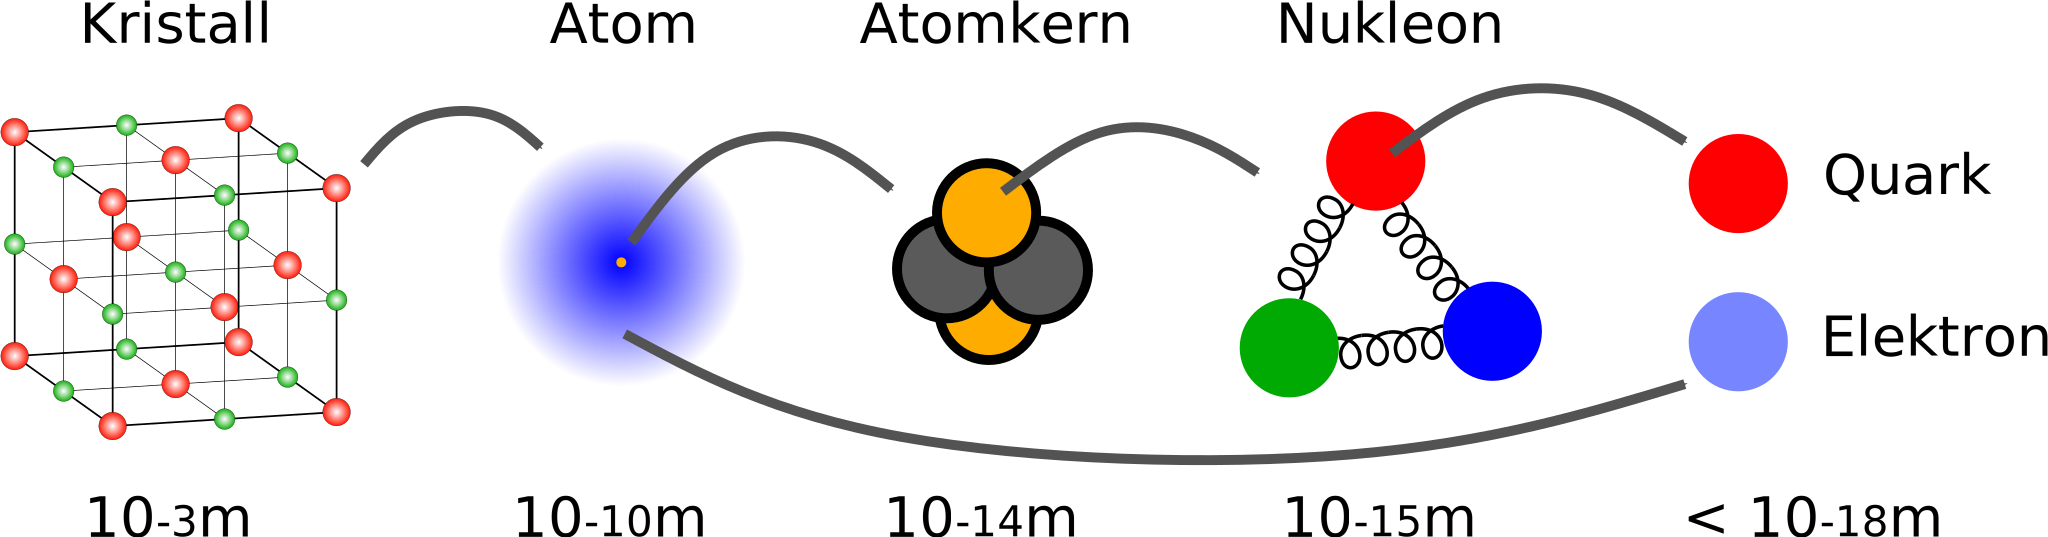
\includegraphics[width=\textwidth]{images/route}
  \end{center}
\end{frame}

\begin{frame}{Das Standardmodell der Teilchenphysik}
  \begin{columns}
    \column{.5\linewidth}
    \scalebox{1}{
    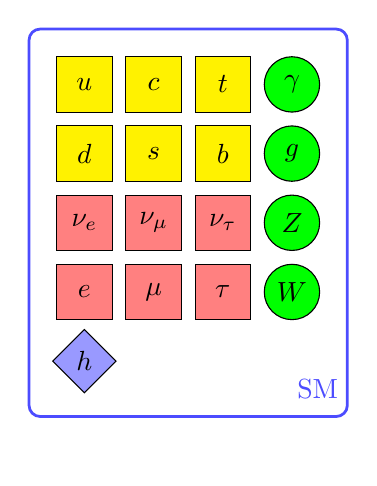
\begin{tikzpicture}[node distance = 2.5em, auto]
      \node[quark] (u) {$u$};
      \node[quark, below of=u] (d) {$d$};
      \node[quark, right of=u] (c) {$c$};
      \node[quark, below of=c] (s) {$s$};
      \node[quark, right of=c] (t) {$t$};
      \node[quark, below of=t] (b) {$b$};
      \node[lepton, below of=d] (ne) {$\nu_e$};
      \node[lepton, below of=ne] (e) {$e$};
      \node[lepton, right of=ne] (nm) {$\nu_\mu$};
      \node[lepton, below of=nm] (m) {$\mu$};
      \node[lepton, right of=nm] (nt) {$\nu_\tau$};
      \node[lepton, below of=nt] (ta) {$\tau$};
      \node[gauge, right of=t] (gamma) {$\gamma$};
      \node[gauge, below of=gamma] (g) {$g$};
      \node[gauge, below of=g] (Z) {$Z$};
      \node[gauge, below of=Z] (W) {$W$};
      \node[phantom, below of=W] (corner) {\phantom{X}};
      \node[phantom, below of=corner] (corner2) {\phantom{X}};
      \draw[line width=1, color=blue!70,rounded corners] ($(u) + (-2em,2em)$) rectangle ($(corner) + (2em,-2em)$);
      \node[color=blue!70, anchor=east] (MSSM) at ($(corner.east) + (1em,-1em)$) {SM};
      \node[scalar, below of=e] (h) {$h$};
    \end{tikzpicture}}
    \column{.5\linewidth}
    \emph{Teilcheninhalt:}\\
    \begin{itemize}
    \item 3 Generationen Fermionen (Quarks und Leptonen)
    \item Eichbosonen (Austauschteilchen)
    \item Higgs-Boson
    \end{itemize}
    \emph{Wechselwirkungen:}\\
    \begin{itemize}
    \item Elektromagnetismus
    \item schwache Wechselwirkung
    \item starke Wechselwirkung
    \end{itemize}
  \end{columns}
\end{frame}

\begin{frame}{Wechselwirkungen}
  Wechselwirkungen beschreiben auf fundamentaler Ebene:
  \begin{itemize}
  \item \emph{Teilchenumwandlung} (Erzeugung, Vernichtung, ``Zerfall'')
  \item \emph{Kraft} zwischen Teilchen (z.B.\ Coulombkraft)
  \end{itemize}
  \begin{align*}
    &\fmfvcenter{escattering} &
    &\fmfvcenter{compton}
  \end{align*}
  \vspace*{1em}
  Wechselwirkungen werden durch \emph{Austauschteilchen} vermittelt
\end{frame}

\begin{frame}{Wechselwirkungen im Standardmodell}
  Wechselwirkungen folgen aus inneren Symmetrien:
  \begin{center}
    \begin{tabular}{lll}
      \toprule
      Symmetriegruppe & Kopplung & Austauschteilchen\\
      \midrule
      $U(1)_Y$  & $g_Y$ & $B$ \\
      $SU(2)_L$ & $g_2$ & $W^1, W^2, W^3$ \\
      $SU(3)_C$ & $g_3$ & $G^1, \dots, G^8$ \\
      \bottomrule
    \end{tabular}
  \end{center}
  Symmetrien werden spontan gebrochen durch Higgs-Feld:
  \begin{center}
    \begin{tabular}{lll}
      \toprule
      Symmetriegruppe & Kopplung & Austauschteilchen\\
      \midrule
      $U(1)_\text{e.m.}$ & $e$ & $\gamma$ \\
      -- & -- & $W^{\pm}$, $Z$ \\
      $SU(3)_C$ & $g_3$ & $G^1, \dots, G^8$ \\
      \bottomrule
    \end{tabular}
  \end{center}
\end{frame}

\begin{frame}{Lagrangedichte des Standardmodells}
  \begin{columns}
    \column{0.6\textwidth}
    \begin{center}
      \includegraphics[width=0.8\textwidth]{images/cup.png}
    \end{center}
    \column{0.4\textwidth}
    zzgl.\ Euler-Lagrange-Gleichungen:
    \begin{align*}
      0 = \frac{\partial\Lagr}{\partial\phi} - \partial_\mu \frac{\partial\Lagr}{\partial(\partial_\mu\phi)}
    \end{align*}
  \end{columns}
\end{frame}

\subsection{Higgsmechanismus}

\begin{frame}{Higgsmechanismus}
  \emph{Ursprüngliches Problem:} Massenterme verletzen die Symmetrien:
  \begin{align*}
    \textcolor{red}{\Lagr_{\text{Elektronmasse}} =
    - m_e \bar{\psi}_e \psi_e \qquad (\text{verboten!})}
  \end{align*}
  $\psi_e =$ Wellenfunktion des Elektrons,\\
  $m_e = 511\,\text{keV}/c^2$ Masse des Elektrons
  \\[1em]
  \emph{Lösung:}\\ \emph{Schritt 1:}
  Neues Feld $\phi$ (Higgs-Feld) einführen und mit Teilchen
  wechselwirken lassen:
  \begin{align*}
    \Lagr_{\text{Higgs}} = - y_e \phi \bar{\psi}_e \psi_e + \cdots
  \end{align*}
  $y_e =$ ``Stärke'' der WW des Elektrons mit Higgs-Feld
\end{frame}

\begin{frame}{Higgsmechanismus}
  \emph{Schritt 2:} Konstruiere Potential, in dem das Higgs-Feld einen
  nicht-trivialen Grundzustand, $v=\text{konst}.$, besitzt:
  \begin{columns}
    \column{0.6\textwidth}
    \begin{center}
      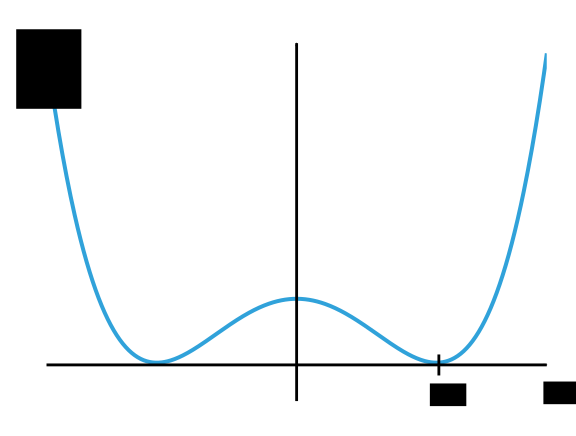
\includegraphics[width=0.9\textwidth]{images/higgs-potential}
    \end{center}
    \column{0.4\textwidth}
    Higgs-Potential:
    \begin{align*}
      V(\phi) = \frac{\lambda}{8}\phi^4 - \frac{\mu^2}{2} \phi^2
    \end{align*}
    Entwickeln von $\phi(x)$ um den Grundzustand:
    \begin{align*}
      \phi(x) = v + h(x)
    \end{align*}
  \end{columns}
\end{frame}

\begin{frame}{Higgsmechanismus}
  Einsetzen von
  \begin{align*}
    \phi(x) = v + h(x)
  \end{align*}
  in $\Lagr_{\text{Higgs}}$ ergibt:
  \begin{align*}
    \Lagr_{\text{Higgs}}
    &= - y_e \phi \bar{\psi}_e \psi_e + \cdots \\
    &= - y_e (v + h(x)) \bar{\psi}_e \psi_e + \cdots \\
    &= - y_e v \bar{\psi}_e \psi_e + \cdots
  \end{align*}
  $\Rightarrow$ durch Ablesen
  \begin{align*}
    m_e = y_e v
  \end{align*}
  Massenterm für Elektron erzeugt durch WW mit Higgs-Feld!\\
  Nebeneffekt: neues Teilchen, \emph{Higgs-Boson} $h$
\end{frame}

\begin{frame}{Higgsmechanismus}
  Mit dem Higgsmechanismus lassen sich die Massen \emph{aller}
  massiven Elementarteilchen generieren, z.B.
  \begin{align*}
    m_e &= y_e v, & m_\mu &= y_\mu v \\
    m_Z^2 &= \frac{v^2}{4}(g_Y^2 + g_2^2) , &  m_W^2 &= \frac{v^2}{4} g_2^2 \\
    m_h^2 &= \lambda v^2
  \end{align*}
  \emph{Vor 2012:}
  Bekannt:
  \begin{align*}
    g_Y &\approx 0.35, &
    g_2 &\approx 0.65, &
    g_3 &\approx 1.2 \\
    v &\approx 245\GeV/c^2, &
    m_h &={} ? &
    \Leftrightarrow \lambda &={} ?, &
  \end{align*}
  \\[1em]
  \emph{2012:} Nachweis des Higgs-Bosons von ATLAS/CMS am LHC
  \begin{align*}
    M_h &= (125.10\pm 0.14) \GeV/c^2 &
    \Rightarrow \ \ \lambda &\approx 0.28
  \end{align*}
\end{frame}

\subsection{Erfolge und Probleme}

\begin{frame}{Erfolge und Probleme des Standardmodells}
  \emph{Erfolge:}
  \begin{itemize}
  \item beschreibt 3 der 4 bekannten Wechselwirkungen
  \item beschreibt uns umgebende sichtbare Materie
  \item viele Präzisionstests bestanden, insbes.\ $(g-2)_e$
  \end{itemize}
  \vspace*{1em}
  \emph{Probleme:}
  \begin{itemize}
  \item beschreibt nicht Gravitation
  \item beschreibt nicht Dunkle Materie, Dunkle Energie
  \item $\approx 3.6\sigma$ Abweichung bzgl.\ $(g-2)_\mu$
  \item [Hierarchie-Problem]
  \end{itemize}
  \vspace*{1em}
  $\Rightarrow$ Das Standardmodell liefert keine vollständige Beschreibung
  des Universums!
\end{frame}

%%%%%%%%%%%%%%%%%%%%%%%%%%%%%%%%%%%%%%%%

\section{Supersymmetrische Erweiterung des Standardmodells}

\begin{frame}{Contents}
  \tableofcontents[currentsection,currentsubsection]
\end{frame}

% \begin{frame}{Contents}
%   \tableofcontents[currentsection]
% \end{frame}

% \subsection{Erweiterung der Raum-Zeit-Symmetrien}

\begin{frame}{Supersymmetrie}
  \emph{Ausgangspunkt:} Die uns umgebende Raumzeit besitzt mehrere
  Symmetrien:
  \begin{itemize}
  \item Raum-Zeit-Translationsinvarianz\\
    $\leftrightarrow$ Erhaltung von Energie- und Impuls $P^\mu$
  \item Rotations-/Boostinvarianz\\
    $\leftrightarrow$ Erhaltung des Drehimpulstensors $M^{\mu\nu}$
  \end{itemize}
  \vspace*{1em}
  \emph{Theorem:} Es gibt nur \emph{eine} Möglichkeit diese Symmetrien
  auf eine nicht-triviale Weise zu erweitern: Supersymmetrie
  \begin{align*}
    |\text{boson}\rangle \leftrightarrow |\text{fermion}\rangle
  \end{align*}
  \emph{Konsequenz:} Zu jedem Teilchen im Standardmodell mit Spin $S$
  korrespondiert ein supersymmetrischer ``Partner'' mit Spin
  $S \pm \frac{1}{2}$.
\end{frame}

\begin{frame}{Minimal Supersymmetrisches Standardmodell}
  \begin{center}
    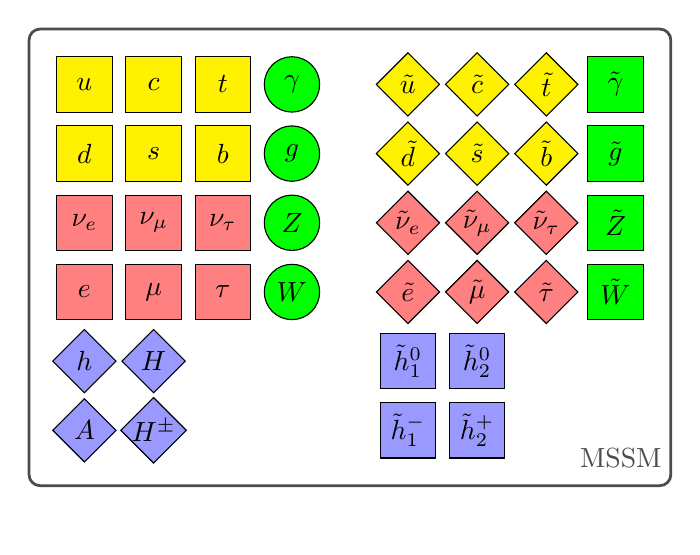
\begin{tikzpicture}[node distance = 2.5em, auto]
        \node[quark] (u) {$u$};
        \node[quark, below of=u] (d) {$d$};
        \node[quark, right of=u] (c) {$c$};
        \node[quark, below of=c] (s) {$s$};
        \node[quark, right of=c] (t) {$t$};
        \node[quark, below of=t] (b) {$b$};
        \node[lepton, below of=d] (ne) {$\nu_e$};
        \node[lepton, below of=ne] (e) {$e$};
        \node[lepton, right of=ne] (nm) {$\nu_\mu$};
        \node[lepton, below of=nm] (m) {$\mu$};
        \node[lepton, right of=nm] (nt) {$\nu_\tau$};
        \node[lepton, below of=nt] (ta) {$\tau$};
        \node[gauge, right of=t] (gamma) {$\gamma$};
        \node[gauge, below of=gamma] (g) {$g$};
        \node[gauge, below of=g] (Z) {$Z$};
        \node[gauge, below of=Z] (W) {$W$};
        \node[scalar, below of=e] (h) {$h$};
        \node[scalar, right of=h] (H) {$H$};
        \node[scalar, below of=h] (A) {$A$};
        \node[scalar, right of=A] (Hpm) {$H^\pm$};
        %
        \node[squark, right=2em of gamma] (su) {$\tilde u$};
        \node[squark, below of=su] (sd) {$\tilde d$};
        \node[squark, right of=su] (sc) {$\tilde c$};
        \node[squark, below of=sc] (ss) {$\tilde s$};
        \node[squark, right of=sc] (st) {$\tilde t$};
        \node[squark, below of=st] (sb) {$\tilde b$};
        \node[slepton, below of=sd] (sne) {$\tilde \nu_e$};
        \node[slepton, below of=sne] (se) {$\tilde e$};
        \node[slepton, right of=sne] (snm) {$\tilde \nu_\mu$};
        \node[slepton, below of=snm] (sm) {$\tilde \mu$};
        \node[slepton, right of=snm] (snt) {$\tilde \nu_\tau$};
        \node[slepton, below of=snt] (sta) {$\tilde \tau$};
        \node[gaugino, right of=st] (sgamma) {$\tilde \gamma$};
        \node[gaugino, below of=sgamma] (sg) {$\tilde g$};
        \node[gaugino, below of=sg] (sZ) {$\tilde Z$};
        \node[gaugino, below of=sZ] (sW) {$\tilde W$};
        \node[higgsino, below of=se] (sh) {$\tilde h_1^0$};
        \node[higgsino, right of=sh] (sH) {$\tilde h_2^0$};
        \node[higgsino, below of=sh] (sA) {$\tilde h^-_1$};
        \node[higgsino, below of=sH] (sHpm) {$\tilde h^+_2$};
        \node[phantom, below of=sW    ] (sZprime) {\phantom{X}};
        \node[phantom, below of=sZprime] (corner) {\phantom{X}};
        \node[phantom, below of=corner] (corner2) {\phantom{X}};
        %
        \draw[line width=1, color=black!70,rounded corners] ($(u) + (-2em,2em)$) rectangle ($(corner) + (2em,-2em)$);
        \node[color=black!70, anchor=east] (SUSY) at ($(corner.east) + (1em,-1em)$) {MSSM};
    \end{tikzpicture}
  \end{center}
\end{frame}

\subsection{Eigenschaften und Probleme}

\begin{frame}{Eigenschaften des MSSM}
  Eigenschaften des MSSM:
  \begin{itemize}
  \item Eichkopplungsvereinigung $\rightarrow$ Möglichkeit die 3 WW zu
    einer zu vereinigen [Bild]
  \item korrekte Vorhersage von $(g-2)_\mu$ [Bild]
  \item Enthält ein Dunkle Materie-Teilchen $\chi^0$
  \item löst das Hierarchie-Problem
  \item Vorhersage der Masse des Higgs-Bosons
  \end{itemize}
\end{frame}

\begin{frame}{Vorhersage der Masse des Higgs-Bosons}
  Higgs-Masse im SM ($\phi(x) = v + h(x)$):
  \begin{align*}
    V(\phi) &= \frac{\textcolor{red}{\lambda}}{8}\phi^4 - \frac{\mu^2}{2} \phi^2 \\
    \Rightarrow
    m_Z^2 &= \frac{1}{4} (g_Y^2 + g_2^2) v^2 \\
    m_h^2 &= \textcolor{red}{\lambda} v^2
  \end{align*}
  Higgs-Masse im MSSM:
  \begin{align*}
    V(\phi) &= \frac{1}{8}\textcolor{red}{\frac{1}{4}\left(g_Y^2 + g_2^2\right)} \cos^2(2\beta) \phi^4 + \cdots \\
    \Rightarrow
    m_Z^2 &= \textcolor{red}{\frac{1}{4}\left(g_Y^2 + g_2^2\right)} v^2 \\
    \Rightarrow
    m_h^2 &= \textcolor{red}{\frac{1}{4}\left(g_Y^2 + g_2^2\right)} v^2 \cos^2(2\beta) = m_Z^2 \cos^2(2\beta)
  \end{align*}
\end{frame}

\begin{frame}{Problem 1: bisher keine SUSY-Teilchen gefunden}
  \begin{center}
    \includegraphics[width=\textwidth]{images/ATLAS_SUSY_Summary}
  \end{center}
\end{frame}

\begin{frame}{Problem 2: Vorhergesagte Higgs-Masse zu klein}
  \begin{align*}
    m_h^2 = m_Z^2 \cos^2(2\beta) \le m_Z^2
  \end{align*}
  Aus den Messungen am LEP und LHC wissen wir jedoch:
  \begin{align*}
    M_h &\approx 125.09 \GeV \\
    M_Z &\approx 91.2 \GeV
  \end{align*}
  $\Rightarrow$ Das MSSM kann nur dann die korrekte Higgs-Masse
  vorhersagen, wenn es große Quantenkorrkturen zwischen $M_h$ und
  $m_h$ gibt!
  \begin{align*}
    M_h^2 &= m_h^2 + \Delta m_h^2
    & &\Rightarrow &
    \Delta m_h^2 &\geq (85\eh{GeV})^2
  \end{align*}
\end{frame}

\subsection{Wie kann man das MSSM testen?}

\begin{frame}{Wie kann man das MSSM testen?}
  \emph{Idee:}
  \begin{enumerate}
  \item Berechne MSSM-Vorhersage von $M_h$ so präzise wie möglich:
  \begin{align*}
    M_h^2 &= m_h^2 + \Delta m_h^2
  \end{align*}
  \item Einschränkung des Parameterraums des MSSM durch Forderung:
    \begin{align*}
      M_h \overset{!}{=} 125.09 \GeV \pm \delta M_h^{\text{exp}} \pm \delta M_h^{\text{theo}}
    \end{align*}
  \end{enumerate}
  \emph{Problem:} Wegen großer Quantenkorrekturen $\Delta m_h^2$:
  \begin{align*}
    \delta M_h^{\text{theo}} &\gtrsim 1\text{--}2\GeV \\
    \delta M_h^{\text{exp}} &= 0.14\eh{GeV} \ \ \mycite{PDG-2019}
  \end{align*}
\end{frame}

%%%%%%%%%%%%%%%%%%%%%%%%%%%%%%%%%%%%%%%%

\section{Präzise Vorhersage der Masse des Higgs-Bosons}

\subsection{Berechnung bis zu endlicher Schleifenordnung}

\begin{frame}{Contents}
  \tableofcontents[currentsection,currentsubsection]
\end{frame}

\begin{frame}{Berechnung bis zu endlicher Schleifenordnung}
  \begin{center}
    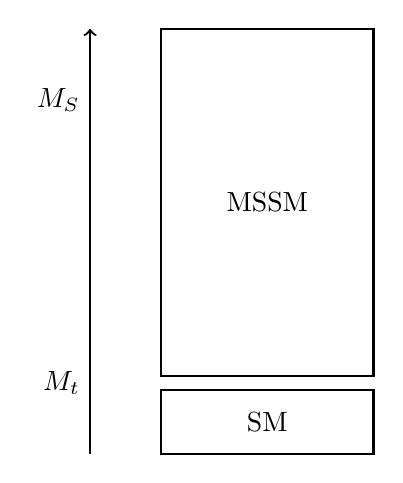
\begin{tikzpicture}[scale=0.9]
      \draw[->, thick] (0,0) -- (0,1) node[left]{$M_t$} -- (0,5) node[left]{$\MS$} -- (0,6);
      \draw[thick] (1,0)   rectangle node{SM}    (4,0.9);
      \draw[thick] (1,1.1) rectangle node{MSSM}  (4,6);
      % \draw[<-, thick, red] (4.1,5) -- (4.5,5) node[right]{$M_h^2 = m_Z^2 c_{2\beta}^2 + \Delta m_h^2$};
      % \draw[<-, thick, darkgreen] (4.1,1) -- (4.5,1) node[right]{$y_f^\MSSM, g_i^\MSSM$};
      % \draw[<->, thick, blue] (4.2,1.2) -- node[right]{RG running} (4.2,4.8);
    \end{tikzpicture}
  \end{center}
\end{frame}

\begin{frame}{Berechnung bis zu endlicher Schleifenordnung}
  Quantenkorrekturen berechnen:
  \begin{align*}
    \fmfvcenter{htop}
  \end{align*}
  \emph{Beobachtung:}
  \begin{itemize}
  \item Quantenkorrekturen lassen sich nach der Anzahl der Schleifen
    sortieren
  \item Jede Schleife hat einen Faktor $\kappa = 1/(4\pi)^2 \approx 1/160$\\
    $\Rightarrow$ Feynman-Diagramm mit $n$-Schleifen hat Faktor $\kappa^n$
  \end{itemize}
  \vspace*{1em}
  \emph{Idee:}
  Reihenentwicklung in Schleifen:
  \begin{align*}
    M_h^2 &= m_Z^2 c_{2\beta}^2 + \Delta m_h^2 \\
    \Delta m_h^2 &= \kappa^1 \Delta_1 + \kappa^2 \Delta_2 + \kappa^3 \Delta_3 + \cdots
  \end{align*}
\end{frame}

\begin{frame}{Los geht's! 1-Schleifen-Quantenkorrekturen}
  Quantenkorrekturen zu $M_h$ mit 1 Schleife:
  \begin{align*}
    \kappa^1\Delta_1
    &= \fmfvcenter{htop} + \fmfvcenter{hstop} + \fmfvcenter{hstopA} \\
    &\phantom{={}} + \fmfvcenter{htoptad} + \fmfvcenter{hstoptad} + \cdots \\
    &\approx 6 \kappa y_t^4 v^2 \left(
      \ln\frac{\MS^2}{m_t^2}
      + x_t^2
      - \frac{x_t^4}{12}
    \right) + \cdots
  \end{align*}
  $m_t \approx 173.34\GeV$,
  $x_t \in [-4,4]$ ``Strärke der Mischung der Stops''
\end{frame}

\begin{frame}{1-Schleifen-Quantenkorrekturen}
  \begin{align*}
    \kappa^1\Delta_1 &\approx
    6 \kappa y_t^4 v^2 \left(
      \ln\frac{\MS^2}{m_t^2}
      + x_t^2
      - \frac{x_t^4}{12}
    \right) + \cdots
  \end{align*}
  % $X_t = A_t - \mu/t_\beta$ = stop mixing parameter,
  % $\MS = (m_Q)_{33} = (m_U)_{33}$
  % 24 mt^4 / (16 Pi^2 v^2) (Log[MS^2/mt^2] + Xt^2/MS^2 - Xt^4/(12 MS^4))
  \\[1em]
  \emph{Beobachtungen:}
  \begin{itemize}
  \item logarithmisch verstärkt mit $L\equiv\ln(\MS / m_t)$
  \item maximal für $x_t \approx \sqrt{6}$
  \item extrem sensitiv auf Wert von $y_t$
  \item damit $M_h \approx 125\eh{GeV}$ muss $\MS \gtrsim 2\TeV$
  \item verbleibende Unsicherheit: $\delta M_h \approx \pm 10 \GeV$
  \end{itemize}
  \vspace*{1em}
  Nicht gut genug!
\end{frame}

\begin{frame}{Weiter geht's! 2-Schleifen-Quantenkorrekturen}
  \includegraphics[width=0.6\textwidth]{images/atas}\\[1em]
  \includegraphics[width=\textwidth]{images/atat}
  \\
  \vspace*{1em}
  \mycite{hep-ph/0105096, hep-ph/0112177}
\end{frame}

\begin{frame}{2-Schleifen-Quantenkorrekturen}
  \begin{align*}
    \kappa^2\Delta_2 &\approx
    \kappa^2 y_t^4 g_3^2 \left(
      c_1 L^2
      + c_2 L
      + c_3
    \right) + \cdots \\
  \end{align*}
  \emph{Beobachtungen:}
  \begin{itemize}
  \item logarithmisch verstärkt mit $L^2$, $L\equiv\ln(\MS / m_t)$
  \item extrem sensitiv auf Wert von $y_t$
  \item verbleibende Unsicherheit: $\delta M_h \approx \pm 3 \GeV$
  \end{itemize}
  \vspace*{1em}
  Immernoch nicht gut genug!
\end{frame}

\begin{frame}{Weiter geht's! 3-Schleifen-Quantenkorrekturen}
  \begin{center}
    \includegraphics[width=0.9\textwidth]{images/h3l-atasas}
  \end{center}
  \mycite{1005.5709}
  \begin{align*}
    \kappa^3\Delta_3 &\approx
    \kappa^3 y_t^4 g_3^4 \left(
      c_7 L^3
      + c_8 L^2
      + c_9 L
      + c_{10}
    \right)
  \end{align*}
  \emph{Beobachtungen:}
  \begin{itemize}
  \item logarithmisch verstärkt mit $L^3$, $L\equiv\ln(\MS / m_t)$
  \item extrem sensitiv auf Wert von $y_t$
  \item verbleibende Unsicherheit: $\delta M_h \approx \pm 1\text{--}2 \GeV$
  \end{itemize}
\end{frame}

\begin{frame}{Konvergenz der Störungsreihe}
  Typische Beträge der Quantenkorrekturen (Abhängig vom Parameterpunkt):
  \begin{align*}
    M_h &= m_h + \kappa^1\Delta_1 + \kappa^2\Delta_2 + \kappa^3\Delta_3 + \cdots \\
    &\approx [91 + O(20\ldots 30) + O(2\ldots 4) + O(1\ldots 2)] \eh{GeV}
  \end{align*}
  \emph{Beobachtungen:}
  \begin{itemize}
  \item große Quantenkorrekturen sind nötig\\
    $\Rightarrow$ $\MS \gtrsim 2\TeV$\\
    $\rightarrow$ Störungsreihe konvergiert schlecht
  \item 4-Schleifen-Quantenkorrekturen aktuell nicht umsetzbar
  \item $\Rightarrow$ verbleibende Unsicherheit durch Abschneiden der
    Störungsreihe: $\delta M_h^{\text{theo}} \approx 1$--$2\GeV$ \\
    zur Erinnerung: $\delta M_h^{\text{exp}} = 0.14\GeV$
  \end{itemize}
\end{frame}

\begin{frame}{Unsicherheitsabschätzung}
  \begin{center}
    \includegraphics[width=0.49\textwidth]{{{plots/SOFTSUSY/SS_TB-20_Xt--sqrt6}}}\hfill
    \includegraphics[width=0.49\textwidth]{{{plots/SOFTSUSY/SS_TB-20_Xt--sqrt6_individual}}}
  \end{center}
  \mycite{1804.09410}
\end{frame}

\begin{frame}{Lösung: Effektive Feldtheorie}
  \emph{Problem:} Abschneiden der Störungsreihe auf 3-Schleifenniveau
  führt zu großen fehlenden Termen:
  \begin{align*}
    \Delta m_h^2\supset c_1 \kappa^1 L^1 + c_2 \kappa^2 L^2 + c_3 \kappa^3 L^3
    + O(\textcolor{red}{\kappa^4 L^4})
  \end{align*}
  \emph{Idee:} Verwende eine Methode, bei der \emph{alle} Terme von der Form
  \begin{align*}
    \Delta m_h^2 \supset \sum_{n=0}^\infty c_n \kappa^n L^n
  \end{align*}
  einbezogen werden:
  \begin{center}
    \emph{Effektive Feldtheorie}
  \end{center}
\end{frame}


\subsection{Berechnung in einer effektiven Feldtheorie}

\begin{frame}{Contents}
  \tableofcontents[currentsection,currentsubsection]
\end{frame}

\begin{frame}{Berechnung in einer effektiven Feldtheorie}
  \emph{Idee:} SUSY-Teilchen entkoppeln an $\MS$ \\
  $\Rightarrow$ SM ist ``effektive Theorie'' (ohne SUSY-Teilchen)\\
  $\Rightarrow$ $\lambda(\MS)$ wird vorhergesagt  \\
  % $\Rightarrow$ effectively: separation of scales $\MS$ and $M_t$.
  \begin{center}
    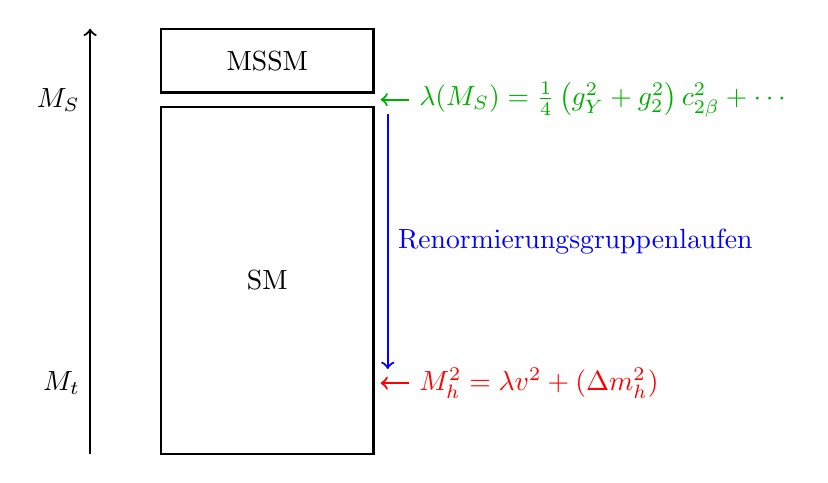
\begin{tikzpicture}[scale=0.9]
      \draw[->, thick] (0,0) -- (0,1) node[left]{$M_t$} -- (0,5) node[left]{$\MS$} -- (0,6);
      \draw[thick] (1,0)   rectangle node{SM}    (4,4.9);
      \draw[thick] (1,5.1) rectangle node{MSSM}  (4,6);
      \draw[<-, thick, darkgreen] (4.1,5) -- (4.5,5) node[right]{$\lambda(\MS) = \frac{1}{4}\left(g_Y^{2} + g_2^2\right) c^2_{2\beta} + \cdots$};
      \draw[<-, thick, red] (4.1,1) -- (4.5,1) node[right]{$M_h^2 = \lambda v^2 + (\Delta m_h^2)$};
      \draw[<-, thick, blue] (4.2,1.2) -- node[right]{Renormierungsgruppenlaufen} (4.2,4.8);
    \end{tikzpicture}
  \end{center}
\end{frame}

\begin{frame}{Summary of EFT approach}
  Typical order of magnitude of loop contributions (depends on
  parameter scenario, here $X_t = 0$, $\MS = 20\eh{TeV}$):
  \begin{align*}
    M_h &= m_h + \Delta m_h^{1\ell} + \Delta m_h^{2\ell} + \Delta m_h^{3\ell} + \cdots \\
    % &= \sqrt{\lambda(M_t)} v + \Delta m_h^{1\ell} + \Delta m_h^{2\ell} + \cdots \\
    &\approx [O(124) + O(0.5\ldots 1) + O(0.1\ldots 0.2) + O(0.02\ldots 0.04)] \eh{GeV}
    % &= \sqrt{\lambda(\MS)} v + \text{logs} + \Delta m_h^{1\ell} + \Delta m_h^{2\ell} + \cdots \\
    % &\approx [O(84) + O(40) + O(0.5\ldots 1) + O(0.1\ldots 0.2)] \eh{GeV}
  \end{align*}
  \emph{Advantages:}
  \begin{itemize}
  \item large logarithmic fixed order loop corrections are avoided
  \item large logarithms $\propto\ln(M_S/M_t)$ are resummed to all orders
  \end{itemize}
  \emph{Disadvantage:} terms of $O(v^2/M_S^2)$ are neglected \\
  $\Rightarrow$ imprecise when $v \sim \MS$ \\
  $\Rightarrow$ large theoretical uncertainty when $v \sim \MS$
\end{frame}

\begin{frame}{Comparison of fixed-order and EFT calculation}
  \begin{center}
    \includegraphics[width=0.49\textwidth]{plots/SOFTSUSY/Mh_MS_TB-20_Xt--sqrt6}\hfill
    \includegraphics[width=0.49\textwidth]{plots/SOFTSUSY/HSSUSY_TB-20_Xt--sqrt6_individual}
  \end{center}
  \mycite{1804.09410}
\end{frame}

%%%%%%%%%%%%%%%%%%%%%%%%%%%%%%%%%%%%%%%%

\section{Wo ist SUSY?}

\begin{frame}{Contents}
  \tableofcontents[currentsection]  
\end{frame}

% \begin{frame}{Wo ist SUSY?}
%   Schwierige Frage!\\[1em]
%   $\rightarrow$ Need to make precise predictions for all parameter scenarios\\[1em]
%   $\rightarrow$ Need to consider all different kinds of EFTs!
% \end{frame}

% \begin{frame}{Scenarios with 1 light Higgs doublet}
%   \begin{center}
%     \begin{tikzpicture}[scale=0.8, every node/.style={transform shape}]
%       \draw[->, thick] (0,0) -- (0,1) node[left]{$M_t$} -- (0,4) node[left]{$\MS$} -- (0,6);
%       \node at (2.5,7) {\emph{I high-scale SUSY}};
%       \draw[thick] (1,0)   rectangle node{SM}    (4,0.9);
%       \draw[thick] (1,1.1) rectangle node{SM}   (4,4.9);
%       \draw[thick] (1,5.1) rectangle node{MSSM}  (4,6);
%       % 
%       \node at (6.5,7) {\emph{II split-SUSY}};
%       \draw[thick] (5,0)   rectangle node{SM}    (8,1.9);
%       \draw[thick] (5,2.1) rectangle node{SM + $\chi_i$ + $\tilde{g}$} (8,4.9);
%       \draw[thick] (5,5.1) rectangle node{MSSM}  (8,6);
%     \end{tikzpicture}
%   \end{center}
% \end{frame}

% \begin{frame}{Scenarios with 2 light/intermediate Higgs doublets}
%   \begin{center}
%     \begin{tikzpicture}[scale=0.8, every node/.style={transform shape}]
%       \draw[->, thick] (0,0) -- (0,1) node[left]{$M_t$} -- (0,4) node[left]{$\MS$} -- (0,6);
%       \node[align=center] at (2.5,7) {\emph{III 2HDM}\\ (light $h_i$, $A$, $H^{\pm}$)};
%       \draw[thick] (1,0)   rectangle node{SM} (4,0.9);
%       \draw[thick] (1,1.1) rectangle node{2HDM} (4,4.9);
%       \draw[thick] (1,5.1) rectangle node{MSSM} (4,6);
%       % 
%       \node[align=center] at (6.5,7) {\emph{IV 2HDM+split}\\ (light $h_i$, $A$, $H^{\pm}$,\\ intermediate $\chi_i$, $\tilde{g}$)};
%       \draw[thick] (5,0)   rectangle node{SM} (8,0.9);
%       \draw[thick] (5,1.1) rectangle node{2HDM} (8,2.9);
%       \draw[thick] (5,3.1) rectangle node[align=center]{2HDM\\ + $\chi_i$ + $\tilde{g}$} (8,4.9);
%       \draw[thick] (5,5.1) rectangle node{MSSM} (8,6);
%       % 
%       \node[align=center] at (10.5,7) {\emph{V 2HDM+split}\\ (light $\chi_i$, $\tilde{g}$, inter-\\ mediate $h_2$, $A$, $H^{\pm}$)};
%       \draw[thick] (9,0)   rectangle node{SM} (12,0.9);
%       \draw[thick] (9,1.1) rectangle node{SM + $\chi_i$ + $\tilde{g}$} (12,2.9);
%       \draw[thick] (9,3.1) rectangle node[align=center]{2HDM\\ + $\chi_i$ + $\tilde{g}$} (12,4.9);
%       \draw[thick] (9,5.1) rectangle node{MSSM} (12,6);
%     \end{tikzpicture}
%   \end{center}
% \end{frame}

\begin{frame}{Wo ist SUSY?}
  \begin{center}
    \includegraphics[width=0.49\textwidth]{plots/Where_is_SUSY/HeavySUSY}\hfill
    \includegraphics[width=0.49\textwidth]{plots/Where_is_SUSY/SplitSUSY}
  \end{center}
  \mycite{1407.4081}
\end{frame}

%%%%%%%%%%%%%%%%%%%%%%%%%%%%%%%%%%%%%%%%

\section{Zusammenfassung}

\begin{frame}{Zusammenfassung}
  \emph{Supersymmetrie} ist eine interessante Erweiterung des
  Standardmodells.  Bietet Erklärungen für Dunkle Materie,
  $(g-2)_\mu$, uvm.
  \\[1em]
  \emph{Präzise Vorhergesagte der Masse des Higgs-Bosons} erlaubt
  Einschränkung des Parameterraums des MSSM.
  \\[1em]
  \emph{Stopmassen} $\MS \gtrsim 2\TeV$ im MSSM nötig für korrekte
  Vorhersage $M_h = 125.09\GeV$.
  \\[1em]
  \emph{Effective Feldtheorie} ist nötig um präzise Vorhersagen zu
  erhalten, da unendliche Reihe großer Logarithmen aufsummiert
\end{frame}

\begin{frame}{Ausblick}
  \begin{center}
    \LARGE Riesiger Zoo an SUSY-Modellen\\ $\Rightarrow$ Automatisierung nötig!
  \end{center}
  \begin{center}
    \includegraphics[width=0.9\textwidth]{images/FS.png}
  \end{center}
\end{frame}

\begin{frame}{Approaches to predict $M_h$}
  \begin{center}
    \begin{tikzpicture}[scale=0.9]
      \draw[->, thick] (0,0) -- (0,1) node[left]{$M_t$} -- (0,5) node[left]{$\MS$} -- (0,6);
      \node at (2.5,7) {\emph{Fixed order}};
      \draw[thick] (1,0)   rectangle node{SM}    (4,0.9);
      \draw[thick] (1,1.1) rectangle node{MSSM}  (4,6);
      \draw[<-, thick, red] (4.1,5) -- (4.5,5) node[right]{$M_h$};
      \node at (7.5,7) {\emph{Effective Field Theory}};
      \draw[thick] (6,0)   rectangle node{SM}    (9,0.9);
      \draw[thick] (6,1.1) rectangle node{EFT}   (9,4.9);
      \draw[thick] (6,5.1) rectangle node{MSSM}  (9,6);
      \draw[<-, thick, red] (9.1,1.5) -- (9.5,1.5) node[right]{$M_h$};
    \end{tikzpicture}
  \end{center}
\end{frame}

% \begin{frame}{EFT avoids large logarithmic corrections}
%   \begin{enumerate}
%   \item Calculate $\lambda$ from the condition ($p^2 = v^2 = 0$):
%     \begin{align*}
%       \partial_{p^2}^{(k)}\Gamma_{h,\ldots,h}^{\MSSM,(n)}
%       = \partial_{p^2}^{(k)}\Gamma_{h,\ldots,h}^{\SM,(n)}
%     \end{align*}
%     $\Rightarrow$
%     \begin{align*}
%       \lambda(Q) &= \frac{1}{4}\left[g_Y^{2} + g_2^2\right] c^2_{2\beta}
%                    + \Delta \lambda^{1\ell} + \Delta \lambda^{2\ell} + \cdots \\
%                  &= \frac{1}{4}\left[g_Y^{2} + g_2^2\right] c^2_{2\beta}
%       + \frac{12 m_t^2 y_t^2}{(4\pi)^2 v^2} \left[
%         \ln\frac{\MS^2}{Q^2} + \frac{X_t^2}{\MS^2} - \frac{X_t^4}{12 \MS^4}
%       \right]
%       + \cdots
%     \end{align*}
%     $\Rightarrow$ \textcolor{darkgreen}{no large logs for $Q\approx\MS$}
%   \item RG running of $\lambda$ from $Q = \MS$ $\rightarrow M_t$.\\
%     $\Rightarrow$ \textcolor{darkgreen}{logs are resummed to all orders}
%   \item Calculate $M_h$ in the SM at $Q = M_t$:
%     \begin{align*}
%       (M_h^\SM)^2 &= \lambda(Q) v^2 + \frac{12 m_t^2 y_t^2}{(4\pi)^2 v^2} \ln\frac{Q^2}{m_t^2} + \cdots
%     \end{align*}
%     $\Rightarrow$ \textcolor{darkgreen}{no large logs for $Q\approx M_t$}
%   \end{enumerate}
% \end{frame}

%%%%%%%%%%%%%%%%%%%%%%%%%%%%%%%%%%%%%%%%
% backup slides
%%%%%%%%%%%%%%%%%%%%%%%%%%%%%%%%%%%%%%%%

\begin{frame}[noframenumbering]
  \begin{center}
    \Huge Backup
  \end{center}
\end{frame}

%%%%%%%%%%%%%%%%%%%%%%%%%%%%%%%%%%%%%%%%

\begin{frame}[noframenumbering]{Higgs masses in the SM}
  Higgs potential
  \begin{align*}
    V_{\text{Higgs}} = -\mu^2 |\Phi|^2 + \frac{\lambda}{2}|\Phi|^4
    = -\frac{\mu^2}{2} (v+h)^2 + \frac{\lambda}{8} (v+h)^4 + \cdots
  \end{align*}
  where
  \begin{align*}
    \Phi =
    \begin{pmatrix}
      0 \\ \frac{1}{\sqrt{2}} (v + h)
    \end{pmatrix}
  \end{align*}
  After eliminating $\mu^2$:
  \begin{align*}
    V_{\text{Higgs}} = \lambda v^2 \frac{h^2}{2} + \cdots
    \qquad\Rightarrow\qquad
    m_h^2 = \lambda v^2  \qquad \text{(tree-level)}
  \end{align*}
  \emph{Until 2012:} $M_h =\ ?$ $\Leftrightarrow$ $\lambda =\ ?$\\
  \emph{Since 2012:} $M_h \approx 125\eh{GeV}$ $\Rightarrow$ $\lambda \approx 0.26$
\end{frame}

%%%%%%%%%%%%%%%%%%%%%%%%%%%%%%%%%%%%%%%%

\begin{frame}[noframenumbering]{Higgs masses in the (real) MSSM}
  Higgs potential:
  \begin{align*}
    V_{\text{Higgs}} = \frac{1}{8}(g_Y^2 + g_2^2)(|h_1|^2 - |h_2|^2)^2 + \frac{g_2^2}{2}|h_1^\dagger h_2|^2 + \cdots
  \end{align*}
  where
  \begin{align*}
    % h, H, A, H^\pm
    h_1 =
    \begin{pmatrix}
      \frac{1}{\sqrt{2}} (v_1 + h_1^0) \\ 0
    \end{pmatrix}, \qquad
    h_2 =
    \begin{pmatrix}
      0 \\ \frac{1}{\sqrt{2}} (v_2 + h_2^0)
    \end{pmatrix}
  \end{align*}
  After EWSB (if $m_A \gg m_Z$):
  \begin{align*}
    V_{\text{Higgs}} \approx \frac{1}{4}(g_Y^2+g_2^2) v^2 c_{2\beta}^2 \frac{h^2}{2} + \cdots
    = m_Z^2 c_{2\beta}^2 \frac{h^2}{2} + \cdots
    % m_h^2 = \frac{1}{2} \left[
    %   m_Z^2 + m_A^2 - \sqrt{(m_Z^2 + m_A^2)^2 - 4 m_Z^2 m_A^2 \cos^2{2\beta}}
    % \right]
  \end{align*}
  $\Rightarrow$ \emph{prediction}:
  \begin{align*}
    m_h^2 = m_Z^2 \cos^2{2\beta}
    % = \frac{1}{4} (g_Y^2 + g_2^2) v^2 \cos^2{2\beta}
    \leq m_Z^2
    \approx (91.2 \eh{GeV})^2  \qquad \text{(tree-level)}
  \end{align*}
\end{frame}

%%%%%%%%%%%%%%%%%%%%%%%%%%%%%%%%%%%%%%%%


\begin{frame}[noframenumbering]{Where is SUSY?}
  \begin{center}
    \emph{I high-scale SUSY}\\[0.5em]
    \includegraphics[width=0.7\textwidth]{{{plots/Where_is_SUSY/Mhband}}}
  \end{center}
  \mycite{1407.4081}
\end{frame}

\begin{frame}[noframenumbering]{Where is SUSY?}
  \begin{center}
    \emph{IV THDM+split}\\[0.5em]
    \includegraphics[width=0.6\textwidth]{{{plots/THDM/SplitTHDMTHDMTower_MS_MA_Xt-2.44949_TB-10_Mu-M12-M3-2000}}}
  \end{center}
\end{frame}

%%%%%%%%%%%%%%%%%%%%%%%%%%%%%%%%%%%%%%%%

\begin{frame}[noframenumbering]{Current status of (N)MSSM spectrum generators}
  \begin{center}
    \emph{MSSM}\\[0.4em]
    \begin{tabular}{llll}
      \toprule
      Spectrum generator & fixed order & EFT & hybrid \\
      \midrule
      \FH                & 2L & 2L & NNLO + NNLL \\
      \FS                & \textcolor{darkgreen}{3L} & \textcolor{darkgreen}{3L} & \textcolor{darkgreen}{NNLO + NNLL}$^\dagger$ \\
      \SOFTSUSY          & \textcolor{darkgreen}{3L} & -- & -- \\
      \SARAH/\SPheno     & 2L & -- & NNLO + LL \\
      \bottomrule
    \end{tabular}
  \end{center}
  %
  \begin{center}
    \emph{NMSSM}\\[0.4em]
    \begin{tabular}{llll}
      \toprule
      Spectrum generator & fixed order & EFT & hybrid \\
      \midrule
      \FH                & -- & -- & -- \\
      \FS                & 2L$^*$ & -- & \textcolor{darkgreen}{NNLO + NNLL}$^\dagger$ \\
      \SOFTSUSY          & 2L$^*$ & -- & -- \\
      \SARAH/\SPheno     & 2L & 1L & NNLO + LL \\
      \bottomrule
    \end{tabular}
  \end{center}
  $^\dagger$ in preparation\\
  $^*$ $O(\at^2)$ corrections in the MSSM limit, no $O(\at\lambda^2)$ corrections
\end{frame}

%%%%%%%%%%%%%%%%%%%%%%%%%%%%%%%%%%%%%%%%

\begin{frame}[noframenumbering]{Uncertainty estimate of the fixed-order \DRbarp\ calculation}
  Calculation of $m_t$ in two different ways as proposed in
  \bigcite{1609.00371}:
  \begin{align*}
    m_t^{[1]} &=
                M_t + \widetilde{\Sigma}_t^{(1L),S} +
                M_t \left[
                \widetilde{\Sigma}_t^{(1L),L} +
                \widetilde{\Sigma}_t^{(1L),R}
                \right] \\
              &\phantom{={}} + M_t
                \left[\widetilde{\Sigma}_t^{(1L),\SQCD}
                + \widetilde{\Sigma}_t^{(2L),\SQCD}
                + \left(\widetilde{\Sigma}_t^{(1L),\SQCD}\right)^2
                \right]\\
    m_t^{[2]} &=
                M_t + \widetilde{\Sigma}_t^{(1L),S} +
                m_t \left[
                \widetilde{\Sigma}_t^{(1L),L} +
                \widetilde{\Sigma}_t^{(1L),R}
                \right] \nonumber \\
              &\phantom{={}} +
                m_t
                \left[\widetilde{\Sigma}_t^{(1L),\SQCD} +
                \widetilde{\Sigma}_t^{(2L),\SQCD}
                \right]
  \end{align*}
  Calculation of $\as$ and $\aem$ in two different ways:
  \begin{align*}
    \as^{[1]}  &= \frac{\as^{\SM(5)}}{1 - \Delta^{(1L)}\as - \Delta^{(2L)}\as}\\
    \as^{[2]}  &= \as^{\SM(5)} \left[1 + \Delta^{(1L)}\as + (\Delta^{(1L)}\as)^2 + \Delta^{(2L)}\as\right]
  \end{align*}
\end{frame}

%%%%%%%%%%%%%%%%%%%%%%%%%%%%%%%%%%%%%%%%

\begin{frame}[noframenumbering]{Uncertainty estimate of FlexibleEFTHiggs-1L}
  \begin{align*}
    \DMhQpole &= \max_{\Qpole\in[M_t/2,2M_t]}\left|M_h(\Qpole) - M_h(M_t)\right| & \text{\mycite{1609.00371}} \\
    \DMhQmatch &= \max_{\Qmatch\in[\MS/2,2\MS]}\left|M_h(\Qmatch) - M_h(\MS)\right| & \text{\mycite{1407.4081}} \\
    \DMhHSSUSYytSM &= \left| M_h(y_t^{\SM,(2L)}(M_Z)) - M_h(y_t^{\SM,(3L)}(M_Z)) \right| & \text{\mycite{1504.05200}} \\
    \DMhEFT &= 0 \quad \text{(has no EFT uncertainty!)} & \text{\mycite{1609.00371}}
  \end{align*}
\end{frame}

%%%%%%%%%%%%%%%%%%%%%%%%%%%%%%%%%%%%%%%%

\begin{frame}[noframenumbering]{Uncertainty estimate of fixed-order \DRbarp\ calculation}
  In \bigcite{1804.09410} 5 sources of uncertainty were combined:
  \begin{align*}
    \DMhQpole &= \max_{\Qpole\in[\MS/2,2\MS]}\left|M_h(\Qpole) - M_h(\MS)\right| & \text{\mycite{1609.00371}} \\
    \DMhQmatch &= \max_{\Qmatch\in[M_Z/2,2M_Z]}\left|M_h(\Qmatch) - M_h(M_Z)\right| & \text{\mycite{\underline{1804.09410}}} \\
    \DMhMt &= \left|M_h(m_t^{[1]}) - M_h(m_t^{[2]})\right| & \text{\mycite{1609.00371}} \\
    \DMhAlphaS &= \left| M_h(\as^{[1]}) - M_h(\as^{[2]}) \right| & \text{\mycite{\underline{1804.09410}}} \\
    \DMhAlphaEm &= \left| M_h(\aem^{[1]}) - M_h(\aem^{[2]}) \right| & \text{\mycite{\underline{1804.09410}}}
  \end{align*}
  Combination:
  \begin{align*}
    \DMh &= \DMhQpole + \DMhQmatch + \DMhMt + \DMhAlphaS + \DMhAlphaEm 
  \end{align*}
\end{frame}

%%%%%%%%%%%%%%%%%%%%%%%%%%%%%%%%%%%%%%%%

\begin{frame}[noframenumbering]{Uncertainty estimate of the EFT calculation}
  In \bigcite{1804.09410} 5 sources of uncertainty were combined:
  \begin{align*}
    \DMhQpole &= \max_{\Qpole\in[M_t/2,2M_t]}\left|M_h(\Qpole) - M_h(M_t)\right| & \text{\mycite{1609.00371}} \\
    \DMhQmatch &= \max_{\Qmatch\in[\MS/2,2\MS]}\left|M_h(\Qmatch) - M_h(\MS)\right| & \text{\mycite{1407.4081}} \\
    \DMhHSSUSYytSM &= \left| M_h(y_t^{\SM,(2L)}(M_Z)) - M_h(y_t^{\SM,(3L)}(M_Z)) \right| & \text{\mycite{1504.05200}} \\
    \DMhEFT &= \left| M_h - M_h(v^2/\MS^2) \right| & \text{\mycite{1504.05200}} \\
    \DMhHSSUSYytMSSM &= \left| M_h - M_h(y_t^\MSSM(\MS)) \right| & \text{\mycite{Bagnaschi,AV,Weiglein}}
  \end{align*}
  Combination:
  \begin{align*}
    \DMhHSSUSY &= \DMhQpole + \DMhQmatch + \DMhHSSUSYytSM + \DMhHSSUSYytMSSM \\
    &\quad + \DMhEFT
  \end{align*}
\end{frame}

%%%%%%%%%%%%%%%%%%%%%%%%%%%%%%%%%%%%%%%%

\begin{frame}[noframenumbering]{Effect of the 3-loop $O(\at\as^2)$ corrections to $M_h$}
  \begin{center}
    \includegraphics[width=0.49\textwidth]{plots/SOFTSUSY/Mh_2L_vs_3L_MS_TB-20_Xt--sqrt6}\hfill
    \includegraphics[width=0.49\textwidth]{plots/Mh3L/scan_Mh_MS_TB-20_Xt--sqrt6_uncertainty_Qpole}
  \end{center}
  \mycite{1708.05720}
\end{frame}

%%%%%%%%%%%%%%%%%%%%%%%%%%%%%%%%%%%%%%%%

\begin{frame}[noframenumbering]{Effect of the 3-loop corrections to $\lambda(\MS)$}
  3-loop corrections to $\lambda(\MS)$ allow for an N$^3$LL
  resummation of strong corrections $O(\at^2\as^2)$:
  \begin{center}
    \includegraphics[width=0.49\textwidth]{plots/HSSUSY-3L/scan_Mh_MS_TB-10_Xt--sqrt6}\hfill
    \includegraphics[width=0.49\textwidth]{plots/HSSUSY-3L/scan_Mh_MS_TB-10_Xt--sqrt6_diff}
  \end{center}
  \mycite{1807.03509}
\end{frame}

%%%%%%%%%%%%%%%%%%%%%%%%%%%%%%%%%%%%%%%%

\begin{frame}[noframenumbering]{Fixed-order vs.\ hybrid calculation in the NMSSM}
  \begin{center}
    \includegraphics[width=0.4\textwidth]{{{plots/NMSSMEFTHiggs/DMh_MS_TB-5_Xt-0_lam-0.1_kap-0.1}}}%\hfill
    \includegraphics[width=0.4\textwidth]{{{plots/NMSSMEFTHiggs/DMh_MS_TB-5_Xt-0_lam-0.3_kap-0.3}}}\\
    \includegraphics[width=0.4\textwidth]{{{plots/NMSSMEFTHiggs/DMh_MS_TB-5_Xt--2_lam-0.1_kap-0.1}}}%\hfill
    \includegraphics[width=0.4\textwidth]{{{plots/NMSSMEFTHiggs/DMh_MS_TB-5_Xt--2_lam-0.3_kap-0.3}}}
  \end{center}
\end{frame}

%%%%%%%%%%%%%%%%%%%%%%%%%%%%%%%%%%%%%%%%

\begin{frame}[noframenumbering]{Gauge Coupling Unification}
  \includegraphics[width=\textwidth]{images/MSSM_gauge_couplings_largeMX}
\end{frame}

\end{document}
